\documentclass[a4paper, fontsize=9pt, twocolumn]{scrreprt}

\setlength{\paperheight}{297mm}
\setlength{\paperwidth}{210mm}
\setlength{\textheight}{252mm}
\setlength{\textwidth}{172mm}
\setlength{\columnsep}{8mm}
\setlength{\headheight}{0mm}
\setlength{\voffset}{-12mm}
\setlength{\hoffset}{0mm}
\setlength{\marginparwidth}{0mm}
\setlength{\parindent}{1pc}
\setlength{\topmargin}{-5mm}
\setlength{\oddsidemargin}{-6mm}
\setlength{\evensidemargin}{-6mm}


\usepackage[utf8]{inputenc}
\usepackage[sc]{mathpazo}
\linespread{1.05}
\usepackage{helvet}
\usepackage{fullpage}

\usepackage{amsmath,amsthm,amssymb}
\usepackage[shortlabel]{enumitem}
\usepackage{nicefrac}
\usepackage{upgreek}
\usepackage{graphicx}
\graphicspath{{figs/figS02/}}



\newcommand{\vect}[1]{\mathrm{\mathbf{#1}}}
\newcommand{\R}{\mathbb R}
\newcommand{\E}{\mathbb E}

\newcommand{\vx}{\vect x}
\newcommand{\vr}{\vect r}
\newcommand{\vu}{\vect u}
\newcommand{\vv}{\vect v}
\newcommand{\vS}{\vect S}
\newcommand{\vX}{\vect X}
\newcommand{\vC}{\vect C}
\newcommand{\vR}{\vect R}
\newcommand{\vW}{\vect W}
\newcommand{\vomega}{\boldsymbol{\upomega}}
\newcommand{\Real}{\text{Re}}

\newcommand{\hvx}{\hat \vx}
\newcommand{\hvX}{\hat \vX}

\DeclareMathOperator{\proj}{proj}
\DeclareMathOperator{\Cov}{Cov}

\usepackage[]{xcolor}
\newcommand{\todo}[1]{{\color{red}\textbf{To do:} #1}}

\usepackage[backend=biber,style=apa,isbn=false,url=false]{biblatex}
\addbibresource{bibliography.bib}
\renewcommand*{\bibfont}{\footnotesize}
\setlength\bibitemsep{0em}

\renewcommand*{\thechapter}{S\arabic{chapter}}

\title{%
    Cosine Contours\\%
    A multipurpose representation \\ for melodies\\[2em]%
    \textsc{supplementary materials}
}
\author{Bas Cornelissen, Willem Zuidema \& John Ashley Burgoyne}
\date{}

\begin{document}

\maketitle
\newpage

\pagebreak



%=============================
\chapter{Random walk baseline}
%=============================



\hspace{-2em}
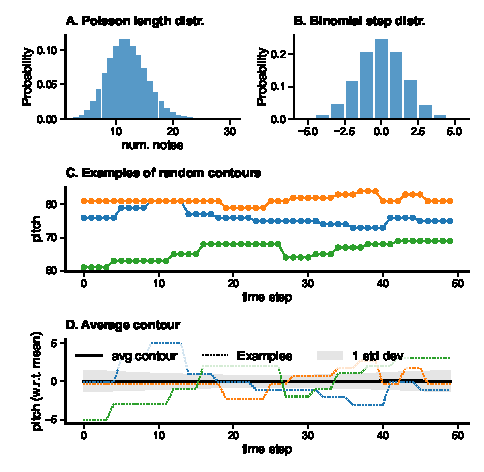
\includegraphics[width=.5\textwidth]{figs/figS01a.pdf}

\noindent
We compared the principal components of phrases to a random walk baseline that was intended to be fairly similar to actual phrase contours.
First, we draw the length (number of notes) $K$ of the random walk from a Poisson distribution with mean $\lambda=12$ (truncated below 3). The value $12$ was chosen so as to approximate the length distribution of phrases. 
Then we draw an initial pitch $x_0$ uniformly between 60 and 85 (in MIDI pitch space).
Next, at every step $k$ we draw the size of a step $r_k$ (the interval) from a Binomial distribution with parameters $n=10$ and $p=0.5$, shifted to have mean 0, and let the next pitch be $x_k = x_{k-1}+r_k$.
We constrain the step sizes to lie between $-12$ and $+12$, meaning that jumps cannot exceed an octave.
This results in small, approximately normally distributed step sizes.
This process yields a sequence of pitches $x_0, \dots, x_{K-1}$.
As usual, we interpolate a step function through these pitches and sample $N=100$ equally spaced pitches to obtain a random contour.
In the figure above we use $N=50$ for readability.
\vfill\pagebreak

\hspace{-2em}
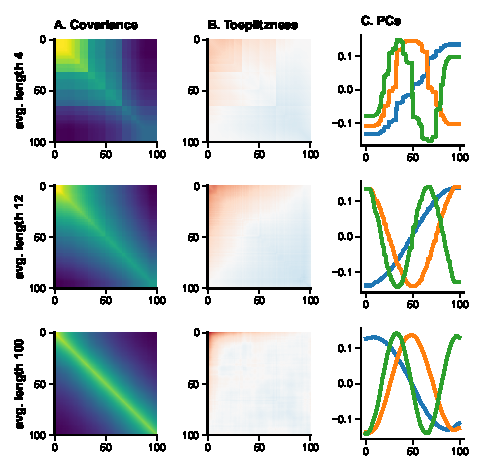
\includegraphics[width=.5\textwidth]{figs/figS01b.pdf}

\noindent
Here we vary the average length $\lambda$ of the random walk baseline.
This affects the number of notes $K$, but we still have $N=100$ throughout.
We generate 10,000 random contours, and compute the covariance matrices (A).
The longer the melodies (larger $K$), the more the covariance matrix starts to resemble a Toeplitz matrix, which has constant values along each of its diagonals.
As an ad-hoc measure of \emph{Toeplitzness}, we measure how much every entry of the covariance matrix differs from the mean value on that diagonal. 
For a Toeplitz matrix, that should be zero everywhere: all diagonals are constant, so every entry also equals the mean of that diagonal.
Column (B) makes clear that the covariance matrix differs from a Toeplitz matrix mostly in the upper left corner, which contains the covariance in the first timesteps. 
All this is also reflected in the principal components (C).



%===================================
\chapter{Analyses of other datasets}
%===================================



In this section we visualize the principal components of melodic material from motifs to songs in different traditions.
For every dataset we show:
\begin{enumerate}[label={\textbf{\textsc{\alph*.}}}]
    \item The first four principal components. The first one is usually a flat line (gray), the second a descending shape (blue), the third a convex shape (orange), and the fourth one undulating (green).
    The corresponding cosines are shown as thin dashed lines in the same colors.
    \item The length distribution of the melodic material, where length is measured in quarter notes. For Gregorian chant we assume all notes are quarter notes.
    \item The covariance matrix.
    \item A scatterplot showing the representations of 2000 contours in 2d cosine contour space.
    \item The reconstruction error using the discrete cosine transform compared to a principal component analysis.
\end{enumerate}
It is clear that the cosine approximation is most accurate at the phrase level. 
For very short melodic fragments (such as neumes or syllables), you see clear effects of the typical number of notes.
For example, neumes often have only 2 notes, meaning there is a jump in the middle of the contour. You can see this in the principal components, but also in the covariance matrix.
Such effects are weaker, but sometimes still visible at the phrase level: German folksongs apparently often have durations of 8 quarter notes, with jumps in the middle, or after 2 of 6 quarter notes.
For complete songs, finally, the principal components are often difficult to interpret.
Only for a very large number of songs (such as when combining all chants in GregoBase) does a pattern reminiscent of the cosines emerge.
But for very small datasets, such as those in the Densmore collection, the principal components are very irregular. 


\vfill
\pagebreak

\newcommand{\showdataset}[2]{%
    \subsubsection*{#2}
    \includegraphics{#1}
    \par
}


%———————————————
\section{Motifs}
%———————————————


All motifs come from Gregorian chant (responsories from  CantusCorpus).
\showdataset{motif-responsory-subset-neumes.pdf}{Neumes}
\showdataset{{motif-responsory-subset-syllables.pdf}}{Syllables}
\showdataset{{motif-responsory-subset-words.pdf}}{Words}
\pagebreak


%————————————————
\section{Phrases}
%————————————————


\showdataset{{phrase-erk-phrase-contours.pdf}}{German: Erk}
\showdataset{{phrase-han-phrase-contours.pdf}}{Chinese: Han}
\showdataset{{phrase-liber-antiphons-phrase-contours.pdf}}{Antiphons}
\pagebreak


%————————————————————————
\section{Random segments}
%————————————————————————


\showdataset{{phrase-erk-random-contours.pdf}}{German: Erk}
\showdataset{{phrase-han-random-contours.pdf}}{German: Han}
\showdataset{{phrase-liber-antiphons-random-contours.pdf}}{Antiphons}
\pagebreak


%————————————————————————————
\section{Phrases (continued)}
%————————————————————————————


\showdataset{{phrase-boehme-phrase-contours.pdf}}{German: Boehme}
\showdataset{{phrase-shanxi-phrase-contours.pdf}}{Chinese: Shanxi}
\showdataset{{phrase-liber-responsories-phrase-contours.pdf}}{Responsories}
\pagebreak


%————————————————————————————————————
\section{Random segments (continued)}
%————————————————————————————————————


\showdataset{{phrase-boehme-random-contours.pdf}}{German: Boehme}
\showdataset{{phrase-shanxi-random-contours.pdf}}{Chinese: Shanxi}
\showdataset{{phrase-liber-responsories-random-contours.pdf}}{Responsories}
\pagebreak


%——————————————
\section{Songs}
%——————————————


\showdataset{song-erk.pdf}{German: Erk}
\showdataset{song-han.pdf}{Chinese: Han}
\showdataset{song-gregobase.pdf}{All chants in GregoBase}
\vfill\pagebreak

\section*{~}
\showdataset{song-boehme-altdeutsches-liederbuch.pdf}{German: Boehme}
\showdataset{song-shanxi.pdf}{Chinese: Shanxi}
\vfill\pagebreak


%——————————————————————————
\section{Songs (continued)}
%——————————————————————————


\showdataset{song-densmore-teton-sioux.pdf}{Teton Sioux (Densmore)} 
\showdataset{song-densmore-nootka.pdf}{Nootka (Densmore)}
\showdataset{song-densmore-papago.pdf}{Papago (Densmore)}
\showdataset{song-densmore-menominee.pdf}{Menominee (Densmore)}


%================================
\chapter{Mathematical background}
%================================



In this section we provide some more mathematical background to illustrate why we observe cosine-shaped principal components.
The aim is to make some of the key points a bit more accessible; we refer to \textcite{Jolliffe2002} for a detailed discussion of principal component analysis, to \textcite{Gray2006} for a rigorous treatment of Toeplitz matrices and their limiting behaviour, and to \textcite{Rao1990} for the discrete cosine transform.


\paragraph{Notation}
%-------------------

We write $N$ for the length of a contour, or the number of steps in a random walk, and $M$ denotes the number of contours.
Consider a dataset $\{\vx_1, \dots, \vx_M\}$ of points $\vx_m = (x_{m1}, \dots, x_{MN})$ in $\R^N$.
We denote the sample mean by $\bar \vx$ and the centered data points by $\hat \vx_m$:
\begin{align}
    \bar \vx = \frac{1}{M} \sum_{m=1}^M \vx_m
    \qquad \text{and} \qquad
    \hat \vx_m= \vx_m - \bar \vx,
\end{align}
and both of course live in $\R^N$. 
An $M \times N$ matrix $\vX$ has entries $(\vX)_{m, n} = x_{mn}$, and for $N\times N$ matrices we generally index rows by $n$ and columns by $k$.


%—————————————————————————————
\section{Principal components}
%—————————————————————————————


\paragraph{Maximize projected variance}
%--------------------------------------

The goal of a principal component analysis is to find a subspace of lower dimensionality $D < N$ that maximizes the variance of the data when it is projected on this subspace.
First, we project the data on a one-dimensional subspace spanned by the unit vector $\vu_1 \in \R^N$.
You can think of the projection of $\vx_n$ as a point in the $N$-dimensional ambient space, but we rather treat it as the scalar $\vu_1^T \vx_n$: the coordinate in the one-dimensional subspace. 
The projected data then has mean $\vu_1^T\bar \vx$ and variance 
\begin{align}
    \frac{1}{M} \sum_{m=1}^M \bigl( \vu_1^T \vx_m - \vu_1^T \bar\vx \bigr)^2
    =\vu_1^T \vS \vu_1,
\end{align}
where $\vS$ is the $N\times n$ covariance matrix given by
\begin{align}
    \vS 
        = \frac{1}{M} \sum_{m=1}^M \vx_m - \bar\vx)(\vx_m - \bar\vx)^T
\end{align}
We want to choose $\vu_1$ in such a way that it maximizes the projected variance $\vu_1^T\vS\vu_1$. 
It can be shown, using a Lagrange multiplier, that under the constraint $\|\vu_1\| = 1$, the projected variance is maximized when
\begin{align}
    \label{eq:pca-eigen-vector}
    \vS \vu_1 = \lambda_1 \vu_1
\end{align}
\parencite[see e.g.~]{Jolliffe2002}.
Left-multiplying by $\vu_1^T$, and using that $\vu_1^T \vu_1 = 1$, this is the case when
\begin{align}
    \label{eq:pca-variance}
    \vu_1^T \vS \vu_1 = \lambda_1.
\end{align}
Equation \eqref{eq:pca-eigen-vector} shows that $\vu_1$ must be an eigenvector of the covariance matrix $\vS$ corresponding to eigenvalue $\lambda_1$, which is exactly the projected variance according to \eqref{eq:pca-variance}.
 The first principal component, in short, is the eigenvector of the covariance matrix corresponding to the largest eigenvalue.
The argument can be extended inductively to identify all principal components as eigenvectors of the covariance matrix, ordered according to their eigenvalues.


\paragraph{Minimize reconstruction error}
%----------------------------------------

It should be noted that one can also motivate principal components in another way.
Consider a dataset $\{x_m\in \R^N\}_m$ as before, and a set of basis vectors $\{\vu_1, \dots, v_N\}$ for $\R^N$ with norm 1.
As before, the projection of $\vx$ on the $\vu_n$ is $c_n = \vu_n^T\vx$, and so we can represent $\vx$ as a coordinate vector $(c_0, \dots, c_N)$.
Now suppose we only use the first $D$ coordinates to represent $\vx$, so we get the truncated representation:
\begin{align}
    \tilde\vx = \sum_{i=1}^D c_i \vu_i.
\end{align}
Now measure the \emph{reconstruction error} as 
\begin{align}
    \textsc{mse} = \frac{1}{M}\sum_{m=1}^M (\vx - \tilde \vx)^2
\end{align}
We ask: how should we choose the basis vectors so that the reconstruction error \textsc{mse} is minimized? 
The answer is the same: as the eigenvectors, ranked in descending order \parencite{Rao1990}.


%————————————————————————————————————————
\section{Toeplitz and circulant matrices}
%————————————————————————————————————————


\emph{Toeplitz matrices} are matrices were every diagonal has the same value. 
They are usually indexed as follows:
\begin{align}
    \vect T = 
    \begin{bmatrix}
    t_0     & t_{-1}    & t_{-2}    &\dots  & t_{-(N-1)}\\
    t_1     & t_{0}     & t_{-1}    &       & \\
    t_2     & t_1       &t_0        &       & \vdots\\
    \vdots  &           &           &\ddots & \\
    t_{N-1} &           &           &\dots  &t_0
    \end{bmatrix}
\end{align}
That means that $T_{i, j} = t_{j-i}$.
Before we discuss Toeplitz matrices further, let's focus on the special subset of circulant matrices.
A \emph{circulant matrix} is a Toeplitz matrix where every row equals the previous row, rotated one step to the right:
\begin{align}
    \vC = 
    \begin{bmatrix}
        c_0     & c_1   & c_2   & \dots & c_{N-1} \\
        c_{N-1} & c_0   & c_1   &       & c_{N-2} \\
        c_{N-2} & c_{N-1} & c_0 & \\
        \vdots  &       & \ddots      &&\vdots\\
        &&&c_0&c_1\\
        c_1 &&\dots &c_{N-1}&c_0
    \end{bmatrix}
\end{align}
It is convenient to start indexing at 0 rather than 1, so that we have $\vC_{n, k} = c_{k-n \mod N}$.
We read the subscripts periodically, so that e.g. $c_{N+3} = c_3$.
For circulant matrices, matrix multiplication takes the form of a \emph{circular convolution}: if $\vect y = \vC \vx$, we have
\begin{align}
    \label{eq:circular-matrix-multiplication}
    y_n = \sum_{k=0}^{N-1} c_{k-n} x_k.
\end{align}


\begin{figure}
    \centering
    \includegraphics[width=.5\textwidth]{figs/suppl-fig-roots-of-unity.pdf}
    \caption{The $N$-th roots of unity for $N=5$ are points on the complex unit circle.}
    \label{fig:roots-of-unity}
\end{figure}


\paragraph{Eigenvectors of circulant matrices}
%---------------------------------------------

Suprisingly, all circulant matrices have the same eigenvectors.
These eigenvectors consist of \emph{($N$-th) roots of unity}: the complex numbers $z$ satisfying $z^N = 1$.
The first complex root of unity is
\begin{align}
    \omega = e^{\frac{2\pi i}{N}},
\end{align}
and its powers $\omega^k$ are other roots of unity, since $(\omega^k)^N = (\omega^N)^k = 1$. 
The numbers $\omega^0, \dots, \omega^{N-1}$ can be visualized as evenly spaced points on the unit circle in the complex plane (see figure \ref{fig:roots-of-unity}).
Importantly, these numbers (like the coefficients $c_k$) are periodical: $\omega^{N+k} = \omega^N \cdot \omega^k = \omega^k$. 

This property allows us to show that the $N$ eigenvectors of a circulant matrix are
\begin{align}
    \vomega_n = (\omega^{n \cdot 0}, \dots, \omega^{n\cdot(N-1)}),
 ,\end{align}
for $n=0, \dots, N-1$.
You can verify this directly when $n=0$, since $\vomega_0$ is then an an all-ones vector, but let's consider the general case.
We have to show that $\vC \vomega_n = \lambda_n \vomega_n$ for some constant $\lambda_n$. 
Using \eqref{eq:circular-matrix-multiplication}, we can show that $k$'the entry of the left hand side indeed equals $\lambda_n \omega^{nk}$:
\begin{align}
    (\vC \vomega_n)_k 
        &= \sum_{j=0}^{N-1} c_{j-k} \cdot \omega^{n \cdot j} \\
        &= \omega^{nk} \cdot \sum_{j=0}^{N-1} c_{j-k}  \cdot \omega^{n(j-k)} \\
        &= \omega^{nk} \cdot \underbrace{
            \sum_{j'=0}^{N-1} c_{j'}  \cdot \omega^{n\cdot j'}
        }_{\lambda_n}.
\end{align}
Here we first multiplied by $\omega^{-nk}/\omega^{-nk}$ to align the indices of the coefficients and the powers. 
Then we used the periodicity of the roots of unity to reorder the sum,
so it no longer depends on $k$ and must equal the eigenvalue $\lambda_n$.
The general case is similar.


Summarizing, every $N\times N$ circulant matrix $\vC$ has the same $N$ eigenvectors $\vomega_0, \dots, \vomega_n$, with (different) corresponding eigenvalues:
\begin{align}
    \label{eq:eigen-pair-circulant-matrix}
    \lambda_n 
        &= c_0 \omega^0 + c_1 \omega^{n} \dots c_{N-1} \omega^{n(N-1)} \\
        &=
        \sum_{j=0}^{N-1} c_j e^{\frac{2\pi i \cdot nj}{N}},
\end{align}
for $n=0, \dots, N-1$.
From the second expression one sees that the eigenvalues $(\lambda_0, \dots, \lambda_{N-1})$ are the discrete Fourier transform of $(c_0, \dots, c_{N-1})$.


\paragraph{Real circulant matrices}
%----------------------------------

In the scenario we are interested in, the matrix $\vC$ is real and symmetric, and such matrices have real eigenvalues and eigenvectors.
To see that the eigenvalues are real, first note that a symmetric circulant matrix satisfies the additional constraint $c_k = c_{N-k}$.
Also observe that $\omega^k$ and $\omega^{N-k} = \omega^{-k}$ are each others mirror image in the real axis (see figure \ref{fig:roots-of-unity}).
They have the same real part,
\begin{equation}
    \label{eq:real-part-root-of-unity}
    \Real(\omega^k) = \cos\Bigl( \frac{2\pi k}{N}\Bigr),
\end{equation}
and when adding them, the complex part cancels out: $\omega^k + \omega^{-k}$ lies on the real axis, at the point $2 \Real(\omega^k)$.
This means that
\begin{align}
    \label{eq:sum-symmetric-circulant}
    c_k \omega^k + c_{N-k} \omega^{N-k}
        = 2c_k \Real(\omega^k)
\end{align}
is a real number.
From \eqref{eq:eigen-pair-circulant-matrix} we see that the eigenvalues $\lambda_n$ consist of many such sums: all complex parts cancel out and the eigenvalues are real\footnote{The expression for the eigenvalues is slightly different depending on whether $N$ is odd or even.}


Now we can also choose real eigenvectors: the real part of $\vomega_n$. 
After all, if $\vomega_n$ is an eigenvector for the real eigenvalue $\lambda_n$, so are $\vomega_{-n}$ and $\vv_n = \nicefrac{1}{2}( \vomega_n + \vomega_{-n})$.
By the same argument as before, equations \eqref{eq:sum-symmetric-circulant} and \eqref{eq:real-part-root-of-unity} show that this is a real eigenvector:
\begin{align}
    \vv_n = \Bigl(1, \; \cos \theta, \; \dots, \; \cos N\theta\Bigr), 
    \quad \theta = \frac{2\pi n}{N}.
\end{align}
This is a discrete cosine function consisting of $N$ points, where higher $n$ implies in higher frequencies.
This is illustrated in figure \ref{fig:eigenvectors-symmetric-circulant}.


\begin{figure}
    \centering
    \includegraphics[width=.5\textwidth]{figs/suppl-fig-cosines.pdf}
    \caption{The eigenvectors of a symmetric, circulant matrix are discrete cosine functions with different periods.}
    \label{fig:eigenvectors-symmetric-circulant}
\end{figure}


\paragraph{Toeplitz is asymptotically circulant}
%-----------------------------------------------

The reason circulant matrices are interesting here, is that
Toeplitz matrices can be shown to be asymptotically equivalent to circulant matrices, and that eigenvalues are preserved.
We refer to \textcite{Gray2006} for a detailed discussion of that result.
What this implies is that the eigenvectors of large Toeplitz matrices are well approximated by those of circulant matrices: sinusoidal functions.
That in turn means that approximately Toeplitz covariance matrices (which are real and symmetric) will have cosine-shaped eigenvectors. 


%————————————————————————————————
\section{PCs of random processes}
%————————————————————————————————


We want to end by discussing two examples where Toeplitz covariance structures arise, and we thus would expect cosine eigenvectors, at least asymptotically.


\begin{figure}
    \centering
    \includegraphics[width=.5\textwidth]{figs/suppl-fig-ar1.pdf}
    \caption{The autocovariance matrix for an autoregressive process \textsc{ar}(1) for two values of $\rho$. When $\rho\to 1$ it approximates the discrete cosine transform.}
    \label{fig:ar1}
\end{figure}


\paragraph{Weakly stationary process}
%------------------------------------

Toeplitz matrices arise naturally in the study of weakly stationary processes.
These are random processes where the mean is constant over time, and where the covariance does not change by shifts in time: it only depends on the distance between two time steps.
That is, when $\Cov(x_i, x_j) = K(j-i)$ is some function of $j-i$, and thus results in a Toeplitz covariance matrix.

One example of such a process is a first order autoregressive process \textsc{ar}(1), where
\begin{align}
    x_n = \rho x_{n-1} + r_n,
\end{align}
where $r_n$ is a random step with mean zero and variance $\sigma^2$, and we assume $x_0 = 0$.
It can be shown that this process has mean $E[x_n] = 0$ and variance $\text{Var}[x_t] = \nicefrac{1}{1-\rho^2}$ if $|\rho| < 1$.
In that case, the covariance is
\begin{align}
    \Cov(x_i, x_j) = \frac{\sigma^2}{1-\rho^2} \cdot \rho^{|j-i|}.
\end{align}
This is actually one of the few cases where an analytic expression for the eigenvectors is known, although it is rather complex \parencite{Ray1970,Rao1990}.
Interestingly, one can use this to show that for \textsc{ar}(1) processes, the discrete cosine transform \textsc{dct-ii} becomes equivalent to the `principal component transform' (Karhunen-Loève transform) as $\rho\to 1$ \parencite[section~3.3.2]{Rao1990}.


\paragraph{High-dimensional random walk}
%---------------------------------------

In the limit $\rho \to 1$ one obtains a random walk. 
\textcite{Antognini2018} analyse the principal components of high-dimensional random walks. 
We briefly summarise their results.
Consider a random walk in $\R^M$ with $N$ steps given by 
\begin{equation}
    \vx_n = \vx_{n-1} + \vr_n
    \label{eq:random-walk}
\end{equation}
where $\vr_n$ is a random step drawn from a probability distribution with zero mean and a finite, normalized covariance matrix.
We start from $\vx_0 = \mathbf{0}$ in $\R^M$.


We can express all this as matrix multiplications.
Collect the points $\vx_n$ and steps $\vr_n$ as the rows of the $N \times M$ matrices $\vX$ and $\vR$ respectively.
Let $\vW$ be a $N\times N$ matrix with $1$'s on the diagonal, $-1$'s on the subdiagonal and zeros elsewhere.
This implements the walking mechanism in the sense that $\vW \vX = \vR$, hence
\begin{align}
    \label{eq:random-walk-matrix}
    \vX = \vW^{-1} \vR.
\end{align}
To compute the covariance matrix $\vS$ we need the centered datapoints $\hat\vx_n = \vx_n - \bar \vx_n$.
The centering operation be conveniently expressed as multiplication by the $N \times N$ \emph{centering matrix} $\vect C = \vect I - \frac{1}{M} \vect J$, where  $\mathbf{J}$ is the all-ones matrix.
This gives 
\begin{align}
    \label{eq:hat-X}
    \hat \vX = \vC \vX = \vC \vW^{-1} \vR
\end{align}
and allows us to express the covariance matrix as $\vS = \frac{1}{N} \hat \vX^T \hat \vX$.
Instead of finding the eigenvectors of $\hat \vX^T\hat \vX$, we can look for those of $\hat \vX\hat \vX^T$. 
After all, if $\vu$ is an eigenvector for $\hat \vX^T \hat \vX$ with nonzero eigenvalue $\lambda$, then $\vect v = \hat\vX \vu$ is the corresponding eigenvector for $\hat \vX \hat\vX^T$.


Putting all this together, \textcite{Antognini2018} look for the eigenvalues and eigenvectors of 
\begin{align}
    \label{eq:target}
    \hat \vX \hat \vX^T
        = \vC \vW^{-1} \vR \vR^{T} \vW^{-T} \vC  
\end{align}
where we used symmetry of $\vC$.
Note that this matrix contains the covariance between timesteps, rather than dimensions.
They observe that in the limit of infinte dimensionality $M \to \infty$, we have that $\vR\vR^T$ tends to the $N\times N$ identity matrix.
This allows us to simplify \eqref{eq:target} to
\begin{align}
    \label{eq:target-simple}
    \hat \vX \hat \vX^T
        = \vC \vW^{-1} \vW^{-T} \vC.
\end{align}
Since $\vW$ is a so called banded Toeplitz matrix, and $\vC$ is circulant, the whole expression can be shown to be asymptotically equivalent to a circulant matrix, meaning that the eigenvectors are cosines.
This analysis can be related to melodic contours, when we consider a collection of $M$ contours of length $N$ as one high-dimensional walk through $\R^M$.


%—————————————————
\printbibliography
%—————————————————


\end{document}